% !TEX TS-program = pdfLaTeX+MakeIndex+BibTeX
% !TEX encoding = UTF-8 Unicode

\PassOptionsToPackage{unicode}{hyperref}
\PassOptionsToPackage{naturalnames}{hyperref}

\documentclass[tg]{mdtufsm}

\usepackage[T1]{fontenc}
\usepackage{fix-cm}
\usepackage{microtype} % Nicer text flowing & typography
\usepackage{times, color}
\usepackage[utf8]{inputenc}
\usepackage{graphicx}
\usepackage{amsmath,latexsym,amssymb}
%\usepackage[hidelinks]{hyperref}
\usepackage[hidelinks,
            bookmarksopen=true,linktoc=none,colorlinks=true,
            linkcolor=black,citecolor=black,filecolor=magenta,urlcolor=blue,
            pdftitle={Exploração da Linguagem Rust para o Desenvolvimento de um Path Tracer Paralelo},
            pdfauthor={Yuri Kunde Schlesner},
            pdfsubject={Trabalho de Graduação},
            pdfkeywords={Computação Gráfica, Linguagens de Programação, Programação Paralela, Rust, Path Tracing, Informática, UFSM}
            ]{hyperref}
%\usepackage[brazilian]{babel}

%\usepackage{fontspec}
%\setmainfont{Linux Libertine G}

%%% PAGE DIMENSIONS
\usepackage[inner=30mm,outer=20mm,top=30mm,bottom=20mm]{geometry} 
%\usepackage{epstopdf}
\usepackage{graphicx}
% \geometry{margin=2in} % for example, change the margins to 2 inches all round
% \geometry{landscape} % set up the page for landscape

% \usepackage[parfill]{parskip} % Activate to begin paragraphs with an empty line rather than an indent

%%% PACKAGES
%\usepackage{amsfonts}
%\usepackage{color}
%\usepackage{booktabs} % for much better looking tables
%\usepackage{array} % for better arrays (eg matrices) in maths
%\usepackage{paralist} % very flexible & customisable lists (eg. enumerate/itemize, etc.)
\usepackage{siunitx}
%\usepackage{verbatim} % adds environment for commenting out blocks of text & for better verbatim
\usepackage{listings}
\usepackage{subcaption}
\captionsetup{compatibility=false}
%\usepackage{microtype}
%\usepackage[numbers]{natbib}
%\usepackage{subfig} % make it possible to include more than one captioned figure/table in a single float
% These packages are all incorporated in the memoir class to one degree or another...

\lstdefinelanguage{Rust}{
  %keywords={typeof, new, true, false, catch, function, return, null, catch, switch, var, if, in, while, do, else, case, break},
  keywords={struct, trait, fn, let, box, mut, pub, impl, for, match, const, if, as, enum, static},
  %keywordstyle=\color{blue}\bfseries,
  %ndkeywords={class, export, boolean, throw, implements, import, this},
  ndkeywords={self, str, u32, uint},
  %ndkeywordstyle=\color{darkgray}\bfseries,
  %identifierstyle=\color{black},
  sensitive=true,
  comment=[l]{//},
  morecomment=[s]{/*}{*/},
  %commentstyle=\color{purple}\ttfamily,
  %stringstyle=\color[rgb]{0.0,0.4,0.65}\ttfamily,
  %morestring=[b]',
  morestring=[b]"
}

\lstset{
	basicstyle=\scriptsize\ttfamily,
	tabsize=2,
	frame=single,
	breaklines=true,
	breakatwhitespace=true,
	xleftmargin=0cm,
	xrightmargin=0cm,
	literate=
		{á}{{\'a}}1 {é}{{\'e}}1 {í}{{\'i}}1 {ó}{{\'o}}1 {ú}{{\'u}}1
		{Á}{{\'A}}1 {É}{{\'E}}1 {Í}{{\'I}}1 {Ó}{{\'O}}1 {Ú}{{\'U}}1
		{à}{{\`a}}1 {è}{{\`e}}1 {ì}{{\`i}}1 {ò}{{\`o}}1 {ù}{{\`u}}1
		{À}{{\`A}}1 {È}{{\'E}}1 {Ì}{{\`I}}1 {Ò}{{\`O}}1 {Ù}{{\`U}}1
		{ä}{{\"a}}1 {ë}{{\"e}}1 {ï}{{\"i}}1 {ö}{{\"o}}1 {ü}{{\"u}}1
		{Ä}{{\"A}}1 {Ë}{{\"E}}1 {Ï}{{\"I}}1 {Ö}{{\"O}}1 {Ü}{{\"U}}1
		{â}{{\^a}}1 {ê}{{\^e}}1 {î}{{\^i}}1 {ô}{{\^o}}1 {û}{{\^u}}1
		{Â}{{\^A}}1 {Ê}{{\^E}}1 {Î}{{\^I}}1 {Ô}{{\^O}}1 {Û}{{\^U}}1
		{ã}{{\~a}}1 {Ã}{{\~A}}1 {õ}{{\~o}}1 {Õ}{{\~O}}1
		{ç}{{\c c}}1 {Ç}{{\c C}}1,
	texcl=true,
	%numbers=left,
	showstringspaces=false,
	commentstyle=\normalfont
}

% For Computer Modern:
%\def\Cpp{{C\nolinebreak[4]\hspace{-.05em}\raisebox{.4ex}{\tiny\bf ++}}}
% For Linux Libertine G
\def\Cpp{{C\nolinebreak[4]\raisebox{.20ex}{\small\bf++}}}

%\newcommand{\todo}[1]{\textsf{\color{red}#1}}
\newcommand{\todo}[1]{}
\graphicspath{{./images/}}


%%=============================================================================
%% Trampa para corrigir o bug do hyperref que redefine o caption das figuras e das
%% tabelas, n�o colocando o nome ``Figura'' antes do n�mero do mesmo na lista
%%=============================================================================

\makeatletter

\long\def\@caption#1[#2]#3{%
  \expandafter\ifx\csname if@capstart\expandafter\endcsname
                  \csname iftrue\endcsname
    \global\let\@currentHref\hc@currentHref
  \else
    \hyper@makecurrent{\@captype}%
  \fi
  \@ifundefined{NR@gettitle}{%
    \def\@currentlabelname{#2}%
  }{%
    \NR@gettitle{#2}%
  }%
  \par\addcontentsline{\csname ext@#1\endcsname}{#1}{%
    \protect\numberline{\csname fnum@#1\endcsname ~-- }{\ignorespaces #2}%
  }%
  \begingroup
    \@parboxrestore
    \if@minipage
      \@setminipage
    \fi
    \normalsize
    \expandafter\ifx\csname if@capstart\expandafter\endcsname
                    \csname iftrue\endcsname
      \global\@capstartfalse
      \@makecaption{\csname fnum@#1\endcsname}{\ignorespaces#3}%
    \else
      \@makecaption{\csname fnum@#1\endcsname}{%
        \ignorespaces
        \ifHy@nesting
          \expandafter\hyper@@anchor\expandafter{\@currentHref}{#3}%
        \else
          \Hy@raisedlink{%
            \expandafter\hyper@@anchor\expandafter{%
              \@currentHref
            }{\relax}%
          }%
          #3%
        \fi
      }%
    \fi
    \par
  \endgroup
}

\makeatother

%%% END Article customizations

\title{Exploração da Linguagem Rust para o Desenvolvimento de um \emph{Path Tracer} Paralelo}
\author{Schlesner}{Yuri Kunde}
\course{Curso de Ciência da Computação}
\altcourse{Curso de Ciência da Computação}
\institute{Centro de Tecnologia}
\degree{Bacharel em Ciência da Computação}

\trabalhoNumero{}
\advisor[Profª.]{Drª.}{Charão}{Andrea Schwertner}
\orientadoratrue

\committee[Profª. Drª.]{Augustin}{Iara}{UFSM}
\committee[Prof. Dr.]{Lima}{João Vicente Ferreira}{UFSM}

\date{2}{Dezembro}{2014}

\keyword{Computação Gráfica}
\keyword{Linguagens de Programação}
\keyword{Programação Paralela}
\keyword{Rust}
\keyword{Path Tracing}
\keyword{Gerenciamento de Memória}
\keyword{C++}
\keyword{Traits}

%\date{} % Activate to display a given date or no date (if empty), otherwise the current date is printed

\begin{document}
\maketitle
\makeapprove

\chapter*{Agradecimentos}
Aos meus pais, que me mantiveram no chão durante todos esses anos, e que sempre estiveram presentes me estimulando a progredir.

Aos amigos, vários dos quais provavelmente não irão ler isto por questões de linguagem, por sempre proporcionarem conversas divertidas ou interessantes sobre todos os assuntos, e por estarem sempre atentos quando precisava de um desabafo.

Aos Brasileiros que fizeram intercâmbio comigo em Chicago, por tornar aquele ano uma experiência marcante em minha vida.

À banca pelos comentários construtivos e relevantes, e à minha coordenadora e orientadora Andrea por ter toda essa paciência comigo.

Ao meu colega de trabalho por fazer o melhor com o que há disponível e por entender que não, eu \emph{não} poderia sair durante mais um mês em uma viajem de trabalho enquanto fazia o TG.

Por fim, aos usuários e desenvolvedores no canal IRC \texttt{\#rust} por ajudar na realização do trabalho e por desenvolver a linguagem Rust, sem a qual ele não existiria.

\begin{abstract}
A geração de imagens por computador é uma tecnologia utilizada para inúmeras aplicações.
Tradicionalmente foram utilizadas linguagens como \Cpp\ para escrever sistemas com este fim. \emph{Rust},
uma nova linguagem de sistemas, tem como um de seus objetivos servir este nicho de aplicação. Este
trabalho teve como objetivo re-implementar o renderizador SmallVCM, escrito em \Cpp, utilizando
Rust, a fim de avaliar se esta nova linguagem poderá ser uma alternativa viável no futuro. Foi
realizada a tradução de parte do programa, incluindo um de seus algoritmos de renderização, buscando
manter uma estrutura similar, resultando em um renderizador com funcionalidade suficiente para gerar
imagens iguais ao original utilizando este algoritmo. Testes de desempenho realizados indicaram que
o novo programa consegue gerar estas imagens em menos tempo que o programa original compilado usando
um \emph{back-end} de otimização similar, mesmo sem ter sofrido modificações no algoritmo.
\end{abstract}

\begin{englishabstract}
{Exploration of the Rust Programming Language for the Development of a Parallel Path Tracer}
{Undergraduate Program in Computer Science}
{Computer Graphics, Programming Languages, Parallel Programming, Rust, Path Tracing, Memory Management, C++, Traits}
{December}
{nd}
Computational generation of images is a technology in use for a multitude of applications.
Traditionally, languages such as \Cpp\ have been used to write systems for these kinds tasks.
\emph{Rust}, a new systems programming language, has as one of its goals to also fit this role. This
work had as its goal to re-implement the SmallVCM renderer, originally written in \Cpp, using Rust,
to evaluate if this new language has the potential to be a viable alternative for these tasks. Parts of
the program have been translated, including one of the available rendering algorithms, trying to
maintain a similar program structure, resulting in a renderer with equivalent functionality, capable
of using this algorithm to render images equivalent to the original. Performance profiling of the new
program shows that it is able to generate these image in less time than the original program compiled
with a similar optimization back-end, even whithout having received any algorithm changes.
\end{englishabstract}

\tableofcontents
\listoffigures
\listoftables
%\listofappendix

\setlength{\baselineskip}{1.5\baselineskip}

%	\item[Período de execução:] Setembro de 2014 a Dezembro de 2014
%	\item[Unidades participantes:] ~\\ Curso de Ciência da Computação \\ Departamento de Eletrônica e Computação
%	\item[Área de conhecimento:] Ciência da Computação
%	\item[Linha de Pesquisa:] Computação Gráfica, Linguagens de Programação, Programação Paralela
%	\item[Tipo de projeto:] Trabalho de Conclusão de Curso

\chapter{Introdução}

A \emph{Computação Gráfica} é a área da Ciência da Computação que estuda tópicos relacionados à
criação, análise e manipulação de imagens e conceitos relacionados. Dentre estas, a síntese (ou
renderização) de imagens é onde uma imagem é criada de forma computacional a partir de um modelo
matemático, frequentemente buscando o fotorrealismo. Esta área possui uma vasta quantidade de aplicações
práticas, como por exemplo: na engenharia, durante o projeto de máquinas ou construções; na arquitetura, para
a visualização de espaços; e para entretenimento, em efeitos especiais de filmes ou em jogos 3D.

Como a geração de imagens fotorrealistas envolve essencialmente uma simulação completa da física da
luz, um processo proibitivamente lento e complexo, são utilizados modelos simplificados. No
passado, devido à limitada capacidade computacional disponível, eram utilizadas aproximações
imperfeitas que, embora produzissem imagens atrativas, não eram muito realistas, especialmente no
quesito da aparência das superfícies e de suas interações com a luz. Com o aumento do poder
computacional disponível, vem sendo usados modelos mais fiéis à realidade e que produzem imagens
mais convincentes, algumas vezes indistinguíveis de uma fotografia real.

\emph{Path tracing} é um método de renderização que assume que a luz se comporta como uma partícula
e calcula uma imagem traçando uma série de raios pelos caminhos através dos quais a luz viajaria quando
refletida através de uma cena. Atualmente, é um dos algoritmos mais usados quando são demandadas
imagens com um grau de realismo extremamente alto devido à sua habilidade de simular o
comportamento da luz com relativa precisão. \citep{pharr2010}

No entanto, este realismo vem ao custo de bastante poder de processamento. Mesmo com o avanço
tecnológico de CPUs, a renderização de imagens continua sendo uma tarefa árdua para processadores.
Sistemas de renderização profissionais são quase exclusivamente escritos em \Cpp\ devido ao controle
que proporciona, não geralmente encontrado em linguagens de mais alto nível. Sistemas mais
recentes fazem o uso de GPUs para acelerar a imensa quantidade de cálculos necessária.
Tendo em vista a baixa expressividade de \Cpp\ comparada a estas outras linguagens, torna-se
interessante explorar alternativas que permitam desenvolvimento mais fácil sem sacrificar o
desempenho requerido.

A linguagem de programação Rust \citep{rust} tem como
seu objetivo ser uma união entre linguagens de programação de sistemas e as tidas como ``linguagens
de alto-nível'', focando simultaneamente em alto-desempenho, segurança e expressividade. Ela atinge
isso usando um modelo tradicional de compilação prévia (\emph{ahead of time}), gerando código nativo que executa
sem utilizar uma máquina virtual, e um sistema de tipos
que permite a verificação automática dos usos de ponteiros durante a compilação, eliminando a
possibilidade de acontecerem erros de memória sem introduzir penalidades excessivas de desempenho
ou consumo de memória. Ao mesmo tempo, integra conceitos mais recentes de linguagens de programação
que aumentam sua expressividade e capacidade de facilmente descrever programas complexos.

\section{Objetivos}

\subsection{Objetivo Geral}

O objetivo geral deste trabalho é portar um \emph{path tracer} para a linguagem Rust e, através deste processo,
realizar uma comparação quantitativa e qualitativa entre as versões escritas nesta linguagem e \Cpp, nos aspectos de
desempenho e organização de código, respectivamente. Como base será utilizado o SmallVCM \citep{smallvcm}, um
\emph{path tracer} de pesquisa escrito em \Cpp, escolhido por implementar uma variedade
de algoritmos diferentes de \emph{path tracing}, ser paralelizado utilizando \emph{multi-threading} e por ser relativamente compacto, consistindo de
aproximadamente 3200 linhas de código.

\subsection{Passos de metodologia}
\begin{itemize}
	\item Estudar Rust e o código original do SmallVCM.
	\item Re-escrever uma parte do SmallVCM utilizando Rust, para a realização de
		testes.
	\item Paralelizar a nova versão do renderizador, fazendo uso das funcionalidades de Rust.
	\item Realizar uma comparação de desempenho e expressividade entre as duas versões,
		atentando a possíveis pontos onde a Rust pode ser melhorada.
\end{itemize}

\section{Justificativa}

Rust é uma linguagem relativamente nova e ainda não existe uma quantidade significativa de aplicações gráficas de \emph{path tracing} escritos nela. Porém, dados seus objetivos de oferecer alto desempenho, ser uma linguagem de alto-nível e de eliminar erros de memória, ela tem potencial de se tornar uma boa alternativa para essas aplicações no futuro, tornando mais fácil a manutenção destes sistemas sem impactar seu desempenho. Este trabalho busca validar a linguagem neste domínio e determinar se ela atualmente cumpre estes objetivos de forma adequada.

\chapter{Fundamentos e Revisão de Literatura}

Neste capítulo é dada uma descrição dos conceitos teóricos das áreas de Linguagens de Programação e de Computação Gráfica nas quais o trabalho e as ferramentas nele utilizadas, a linguagem de programação Rust e o algoritmo de \emph{path tracing}, se baseiam.

\section{Rust}

Rust \citep{rust} é uma linguagem de programação multi-paradigma, oficialmente patrocinada pela
Mozilla Research mas, sendo um projeto \emph{open-source}, desenvolvida também por sua comunidade. Ela busca atender as necessidades
de programadores que atualmente utilizariam linguagens como C ou
\Cpp, por questões de desempenho ou de controle sobre o hardware. Uma de suas características mais
distintivas é a utilização de um modelo de referências baseado em regiões \citep{grossman2002}, que
automaticamente gerencia a vida de alocações de memória, evitando que sejam feitos erros neste
gerenciamento, ou que memória inválida seja acessada pelo programa e fazendo isso sem necessitar o uso de um
\emph{garbage collector}. A linguagem, originalmente projetada por Graydon Hoare como um projeto
pessoal, foi adotada pela Mozilla Research afim de servir como linguagem de
implementação do projeto Servo \citep{servo}, um browser experimental de próxima geração, mas
atualmente já cresceu além deste objetivo para se tornar um projeto maior.

Além de melhorias no gerenciamento de memória, a linguagem busca também trazer funcionalidades
tradicionalmente oferecidas em linguagens funcionais à programação procedural, trazendo uma forte inspiração de linguagens
como ML \citep{milner1997} e assim trazendo funcionalidades como \emph{pattern matching} e \emph{algebraic data types}. (Tuplas e \emph{sum types}, também conhecidos como tipos variantes ou uniões discriminadas.) A linguagem não implementa o modelo de herança tradicional de programação orientada a objetos,
oferecendo em troca o conceito de \emph{traits}.

O compilador oficial da linguagem, o rustc, é implementado na própria linguagem e utiliza a
infraestrutura do projeto LLVM \citep{lattner2004}, permitindo que usufrua das capacidades de
otimização e geração de código do projeto para alcançar uma variedade de plataformas. O compilador
também tem suporte ao carregamento de \emph{plugins} durante o processo de análise, o que expõe
poderosas capacidades de meta-programação aos usuários. Alguns exemplos de projetos que utilizam
estas capacidades são o RustGPU \citep{holk2013}, que permite a compilação de código Rust para
execução paralela em GPUs, e Zinc \citep{zinc}, um \emph{framework} para desenvolvimento de
aplicações embarcadas em microprocessadores.

\subsection{\emph{Lifetimes}}

Para criar uma linguagem segura, eficiente e sem \emph{runtime}, é necessário assegurar-se de que todos os ponteiros, ou referências, no programa sejam válidos quando são acessados. Para que isto seja possível sem haver custo durante a execução, esta é uma tarefa que precisa ser feita durante a compilação do programa, e não durante sua execução, como é feito em muitas linguagens onde todos os acessos através de ponteiros são testados por validez antes de serem executados ou onde esta tarefa é deixada a cargo do programador, resultando em eventuais erros.

Rust modela esta restrição fazendo uma análise do fluxo de valores e referências na função, que tem sua vida delimitada por escopos léxicos no programa. É permitido que uma variável seja usada em escopos dentro da qual ela foi definida, e quaisquer referências criadas à esta variável tem seu tipo associado ao escopo, de forma a proibir que estas escapem para um escopo superior onde não seriam mais necessariamente válidas, pois a variável à qual apontam teria sido destruída no fim do seu respectivo escopo. A região na qual uma variável é válida e referências a ela podem existir é chamada de sua \emph{lifetime}.

Para suportar a mobilidade de valores para escopos mais externos, variáveis também podem ser movidas. Mover uma variável (para outra variável; para dentro de uma chamada de função; ou retornando-a para fora de uma função) invalida a variável original que continha o objeto. O compilador proíbe acessos a esta variável após ela ter sido movida, pois seus conteúdos não são mais válidos, como mostrado na \autoref{code:moving-vars}. Por esta mesma razão, é proibido mover uma variável para a qual existam referências, que seriam invalidadas se isto acontecesse. Por isso, o ato de criar uma referência a partir de uma variável é chamado \emph{borrow} (``emprestar''): o direito de vida da variável é compartilhado com a referência, enquanto esta existir.

Existem usos que esta restrição de referências baseada exclusivamente no escopo léxico é muito limitada para expressar. Nestes casos é feito o uso de \emph{variáveis de lifetime}, que permitem que referências sejam retornadas de funções ou armazenadas em estruturas. Uma \emph{lifetime} nomeada é adicionado a uma função, e pode ser usada para especificar que certas referências criadas dentro da função são válidas dentro de um escopo maior que a chamada, correspondendo a um escopo herdado da função que a chamou. Um exemplo do uso desse mecanismo pode ser visto na \autoref{code:named-lifetime}. \citep{rust-lifetimes}

\begin{figure}
	\centering
	\begin{minipage}[c]{0.45\textwidth}
		\begin{lstlisting}[language=Rust]
struct Coisa;

fn foobar() -> Box<Coisa> {
	let a = Coisa; // Alocado na pilha
	let b = box Coisa; // Alocado no heap

	let c = b; // Movido de b para c

	b // ERRO -- Move e tenta retornar b
}
		\end{lstlisting}
		\begin{lstlisting}[numbers=none, breaklines=true]
<anon>:9:5: 9:6 error: use of moved value: `b`
<anon>:7:9: 7:10 note: `b` moved here because it has type `Box<Coisa>`, which is moved by default (use `ref` to override)
<anon>:7     let c = b;
		\end{lstlisting}
		\caption{
			Exemplo do rastreio de validade de variáveis detectando uso de uma variável já movida.
		}
		\label{code:moving-vars}
	\end{minipage}%
	\hspace{2em}%
	\begin{minipage}[c]{0.45\textwidth}
		\begin{lstlisting}[language=Rust]
fn get_first<T, 'a>
		(v: &'a Vec<T>) -> &'a T {
	v[0]
}
		\end{lstlisting}
		\caption[Exemplo de uso de uma \emph{lifetime} nomeada.]{
			Exemplo de uso de uma \emph{lifetime} nomeada. A sintaxe \texttt{'a} é utilizada para introduzir um nome de \emph{lifetime} que é então usado para especificar que a referência retornada pela função tem o mesmo período de validade que a referência passada como parâmetro.
		}
		\label{code:named-lifetime}
	\end{minipage}
\end{figure}

\subsection{Prevenção de \emph{Aliasing}} \label{sect:aliasing}

Para facilitar a análise do comportamento de um programa pelo usuário, Rust também impõe restrições quanto a mutabilidade de referências a objetos. Referências \emph{únicas} ou \emph{mutáveis} permitem a modificação do objeto a que apontam, mas restringem qualquer acesso a ele sem ser pela referência enquanto estiver emprestado. Referências \emph{compartilhadas} ou \emph{imutáveis} restringem a modificação do objeto para a qual apontam, mas permitem a existência de várias delas apontando para o mesmo. Isto garante que, se uma função receber uma referência compartilhada, o objeto a qual ela aponta nunca será modificado durante a execução da função, não precisando o programador ou o compilador preocupar-se com efeitos colaterais de operações em outros objetos. Da mesma forma, se uma função receber uma função única, poderá modificá-la sem se preocupar se isto irá interferir com outros objetos ou referências presentes no programa. Exemplos das situações descritas aqui são mostrados na \autoref{code:aliasing}.

A restrição em \emph{aliasing} também é importante para evitar que referências possam apontar para posições inválidas: ela evita uma classe de problemas causados pela modificação de um objeto enquanto existam referências à objetos contidos nele. Utilizando-se um vetor redimensionável, por exemplo, pode ser criada uma referência à um elemento dentro do vetor. Nesta situação, se então forem permitidas modificações ao vetor, este poderia ser redimensionado de forma a invalidar a referência. \citep{rust-lifetimes}

\begin{figure}
	\centering
	\begin{subfigure}[c]{0.48\textwidth}
	\begin{lstlisting}[language=Rust]
fn main() {
	let mut n = 52u32;

	let a = &n;
	let b = &n; // OK -- Duas referencias somente-leitura

	println!("{} {}", *a, *b);
}
	\end{lstlisting}
	\caption{}
	\label{code:aliasing:shared1}
	\end{subfigure}
	~~~
	\begin{subfigure}[c]{0.48\textwidth}
	\begin{lstlisting}[language=Rust]
fn main() {
	let mut n = 52u32;

	let a = &n;
	let b = &n; // OK -- Duas referências somente-leitura

	// ERRO -- Não pode modificar referência compartilhada
	*a = 24;

	println!("{} {}", *a, *b);
}
	\end{lstlisting}
	\begin{lstlisting}[numbers=none, breaklines=true]
<anon>:8:5: 8:12 error: cannot assign to immutable dereference of `&`-pointer `*a`
<anon>:8     *a = 24;
             ^~~~~~~
	\end{lstlisting}
	\caption{}
	\label{code:aliasing:shared2}
	\end{subfigure}
	\\[2em]
	\begin{subfigure}[c]{0.48\textwidth}
	\begin{lstlisting}[language=Rust]
fn main() {
	let mut n = 52u32;

	let a = &mut n; // OK -- Uma referência mutável

	*a = 24; // OK

	println!("{}", *a);
}
	\end{lstlisting}
	\caption{}
	\label{code:aliasing:mut1}
	\end{subfigure}
	~~~
	\begin{subfigure}[c]{0.48\textwidth}
	\begin{lstlisting}[language=Rust]
fn main() {
	let mut n = 52u32;

	let a = &mut n;
	let b = &n; // ERRO -- n já tem uma referência mutável

	println!("{} {}", *a, *b);
}
	\end{lstlisting}
	\begin{lstlisting}[numbers=none, breaklines=true]
<anon>:5:14: 5:15 error: cannot borrow `n` as immutable because it is also borrowed as mutable
<anon>:5     let b = &n;
                      ^
<anon>:4:18: 4:19 note: previous borrow of `n` occurs here; the mutable borrow prevents subsequent moves, borrows, or modification of `n` until the borrow ends
<anon>:4     let a = &mut n;
                          ^
	\end{lstlisting}
	\caption{}
	\label{code:aliasing:mut2}
	\end{subfigure}
	\caption{Exemplos de uso de referências e restrições de \emph{aliasing}.}
	\label{code:aliasing}
\end{figure}

Esta garantia de que valores só podem ser modificados através de um único ponto por vez também automaticamente assegura que não existam erros de sincronização em programas concorrentes. Dados compartilhados por vários \emph{threads} serão acessados exclusivamente através de referências compartilhadas, com a garantia de que não serão modificados, e assim não precisam de exclusão mútua para evitar condições de corrida. Por outro lado, se um \emph{thread} possuir uma referência única, sabe-se que este dado não pode ser lido em nenhum outro lugar, também evitando a necessidade de sincronismo durante modificações.

\subsection{\emph{Traits}}

O projeto de Rust considera importante o suporte a programação genérica sobre tipos polimórficos, embora não suporte herança de classes. Este suporte é fornecido através do conceito de \emph{traits}. \emph{Traits} são similares aos conceitos de \emph{interfaces} ou \emph{type-classes} \citep{wadler1989}: um tipo apresentando uma interface que consiste apenas de declarações de funções, sem campos de dados ou implementação, e que forma um contrato especificando a interação entre dois componentes do código. Estas funções devem ser posteriormente implementadas por tipos concretos, de acordo com o contrato estabelecido, permitindo que estes tipos sejam usados de forma genérica através da interface. Um dado tipo pode implementar mais de uma interface, permitindo expor vários conjuntos de funcionalidade distintos. \citep{rust-guide} \todo{exemplo}

Uma vantagem de \emph{traits} sobre o modelo de herança tradicional é que se evita a ambiguidade presente em casos onde duas superclasses em de um tipo herdam de uma mesma classe. Isto cria uma ambiguidade onde cada classe pode conter dentro de si uma instância separada dos campos das classes pai ou, alternativamente, onde ambas compartilham os mesmos campos, resultando em uma semântica confusa e difícil de usar corretamente. Esta situação é chamada de ``problema diamante'', devido a estrutura do grafo de herança resultante. Por esta razão, muitas linguagens restringem seu suporte à herança simples, permitindo que classes herdem de somente uma superclasse. \citep{scharli2003}

Outra vantagem é a possibilidade de se estender tipos através da definição posterior de um novo \emph{trait}. Como a implementação de um \emph{trait} para certo tipo é separada da definição do tipo em si, pode-se fazer um tipo pré-existente suportar novas interfaces. \todo{exemplo junto com o 1o?}

\subsection{\texttt{unsafe}}

Caso as limitações anteriormente descritas que são impostas no gerenciamento de memória e em referências mostrem-se muito restritivas durante a implementação de alguma estrutura de dados, algoritmo ou interface com outras bibliotecas ou APIs externas, existe a opção de fazer o uso de um bloco \texttt{unsafe}. Blocos \texttt{unsafe} não alteram a semântica da linguagem, mas relaxam restrições do verificador estático acerca de operações que não garantem a corretude do programa. Foram criados para expandir o campo de aplicação da linguagem, pois permitem que código Rust faça chamadas a funções definidas em outras linguagens (como funções de bibliotecas C ou do SO) e a conversão de referências para ponteiros não restritos. Cabe então ao programador verificar que as operações contidas nestes blocos não violem as invariantes assumidas pelo sistema de tipos. A intenção é que estes blocos sejam utilizados para implementar abstrações seguras por cima das operações necessárias, sendo facilmente identificados para fins de verificação de seu correto funcionamento. \citep{rust-unsafe}

A biblioteca padrão Rust, implementada quase que totalmente na própria linguagem, inclui uma multitude de tipos que utilizam esta estratégia para fornecer contrapartidas checadas em \emph{runtime} das invariantes do sistema de tipos, como ponteiros com contagem de referências (tipo \texttt{Rc<T>}), estruturas de dados e estruturas de concorrência, como o tipo \texttt{Mutex<T>}, que impede que um valor seja acessado sem antes adquirir uma trava de exclusão mútua.

\section{\emph{Path Tracing}}

\emph{Path tracing} faz parte de uma família de algoritmos comumente denominados algoritmos de
\emph{ray tracing}. Embora também utilizados na física e nas engenharias, no contexto deste trabalho
são algoritmos que tem como finalidade a produção de imagens que retratam cenas tridimensionais.

Todos os algoritmos desta família se baseiam na ideia fundamental de simular o comportamento da luz
traçando raios que saem da câmera virtual em direção à cena. Isto é o contrário do que ocorre na
vida real, onde a luz é emitida de uma fonte e viaja pelo espaço até chegar ao observador, mas não
afeta negativamente o resultado final e torna o algoritmo computacionalmente viável, pois assegura
que todo o raio traçado é um que eventualmente chegaria no observador. Pelo contrário, a maioria da luz numa cena
não chega até o observador, que subtende um espaço relativamente pequeno nela, o que geraria um grande número de cálculos desperdiçados. \citep{pharr2010}

Os primeiros algoritmos deste tipo a serem usados simplesmente traçavam um raio por pixel da imagem,
encontrando a intersecção deste raio com a cena e calculando sua aparência de acordo com algum
modelo básico de iluminação. Desta forma, não eram reproduzidas sombras nem superfícies refletivas,
como espelhos ou objetos metálicos. Estes tipo de algoritmos vieram a ser chamado de algoritmos de
\emph{ray casting}.

\Citet{whitted1980} propôs um novo método que soluciona estes problemas. Além do primeiro raio
partindo da câmera, são também traçados raios que vão do ponto sendo iluminado até cada uma das
fontes luminosas, permitindo que cada luz só seja adicionada se não estiver obstruída por outro
objeto e assim permitindo a renderização de sombras. Em superfícies refletivas, outro raio é traçado
na direção do reflexo, o qual é utilizado para calcular a luminosidade naquela direção, da mesma
maneira que o raio inicial. Assim, este algoritmo implementa \emph{ray tracing recursivo}.

\Citet{cook1984} aprimoraram o algoritmo de \citeauthor{whitted1980} para que suporte uma variedade
de efeitos adicionais como superfícies foscas e translúcidas, sombras com penumbras realísticas,
profundidade de campo e borrão de movimento. Todos estes efeitos são realizados através do mesmo
método de tirar várias amostras em cada ponto da imagem, introduzindo uma variação nas direções ou
posições traçadas em cada amostra. Embora não tenha o embasamento matemático, esta é a mesma ideia
básica utilizada posteriormente em algoritmos que utilizam integração Monte Carlo.

\begin{figure}
	\centering
	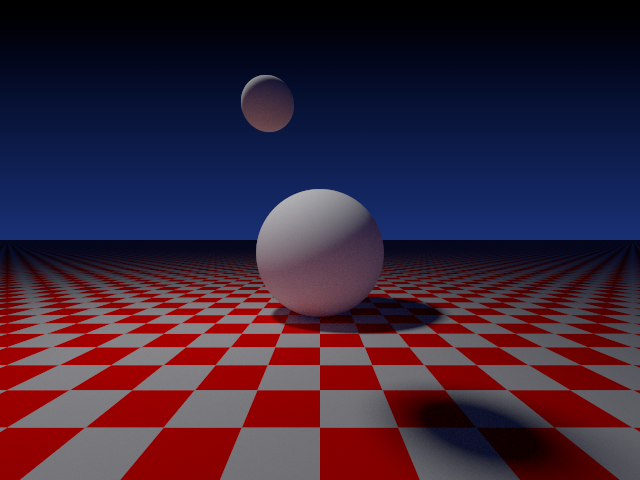
\includegraphics[width=0.5\textwidth]{exemplo_imagem}
	\caption[Um exemplo de uma imagem gerada utilizando \emph{path tracing}.]{
		Um exemplo de uma imagem gerada utilizando \emph{path tracing}. Note como a luz que atinge o
		plano xadrez é refletida de volta para iluminar a esfera, um fenômeno conhecido como
		\emph{iluminação indireta} e que é corretamente simulado pelo algoritmo.
	}
	\label{fig:path_tracing}
\end{figure}

\Citet{kajiya1986} introduz a \emph{equação de renderização}, que descreve a interação da luz com as
superfícies, modelando também a reflexão de luz em superfícies completamente foscas (ver
\autoref{fig:path_tracing}.) Esta serve como uma importante fundação teórica que é usada até hoje
como base
para o cálculo da imagem ou para o desenvolvimento de aproximações. No mesmo artigo é introduzida a
técnica de \emph{path tracing}, que difere das anteriores desenvolvidas por \citeauthor{cook1984} e
\citeauthor{whitted1980} por observar que os raios mais impactantes na aparência final da imagem são
os de baixa profundidade, e assim traçando apenas um raio recursivo por amostra, evitando o
crescimento exponencial do número de raios traçados que ocorre com as outras técnicas.

Embora capaz de produzir imagens extremamente realísticas, \emph{path tracing} pode requerer uma
quantidade impraticável de amostras para renderizar satisfatoriamente certos tipos de cenas onde não
exista uma linha de visão direta entre as superfícies e as fontes de luz. Nestas cenas, a maioria da
iluminação se dá através de caminhos indiretos ou através de superfícies refratantes que projetam
padrões de luz complicados em outras superfícies (conhecidos como \emph{caustics}.) Para contornar
estes problemas foram desenvolvidas inúmeras extensões ao algoritmo de \emph{path tracing}. Dentre
elas se destaca \emph{bidirectional path tracing}, introduzido por \citet{lafortune1993}. Este
algoritmo foi depois reformulado em \citep{veach1997}, onde também foi introduzida a técnica de
\emph{multiple importance sampling} e o algoritmo \emph{Metropolis light transport}.

\section{SmallVCM}

\begin{figure}
	\centering
	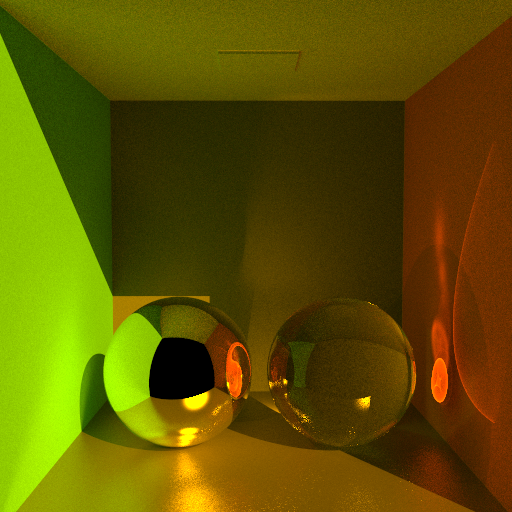
\includegraphics[width=0.5\textwidth]{ggbs_s_vcm}
	\caption[Uma imagem gerada pelo SmallVCM.]{
		Uma imagem gerada pelo SmallVCM utilizando o algoritmo \emph{Vertex Connection and Merging}.
	}
	\label{fig:smallvcm_img}
\end{figure}

SmallVCM \citep{smallvcm} é um renderizador de imagens baseado em algoritmos de \emph{ray tracing} e \emph{path tracing} desenvolvido pelo autor para servir como uma implementação de exemplo de seu algoritmo \emph{Vertex Connection and Merging} \citep{georgiev2012}. Além deste algoritmo, o programa também implementa uma variedade de outros incluindo \emph{ray casting}, \emph{path tracing}, \emph{light tracing}, \emph{bidirectional path tracing} e \emph{photon mapping}. Por ter propósito de educar sobre os algoritmos, não possui funcionalidades avançadas como animação e é limitado a renderizar um pequeno conjunto de cenas de exemplo incluídas no programa. Uma imagem gerada com o programa pode ser vista na \autoref{fig:smallvcm_img}. O programa também possui uma função que gera um relatório de comparação do desempenho relativo de cada algoritmo.

Escrito em \Cpp, o SmallVCM segue uma estrutura de projeto claramente organizada, com seus tipos e funções divididos em arquivos de acordo com sua função principal. As implementações dos algoritmos de renderização são implementadas em classes e arquivos separados, e utilizam o resto da infraestrutura de cena e cálculo do projeto. A partir das opções passadas na linha de comando, é criada uma cena, utilizando um dos modelos disponíveis, e um renderizador, dos quais existem várias implementações para os vários algoritmos. Todos os renderizadores utilizam uma infraestrutura comum de tipos representando os objetos, fontes luminosas e materiais da cena. Os resultados intermediários da renderização são acumulados em um \texttt{Framebuffer} e subsequentemente salvos para um arquivo após terem sido executadas um número especificado de iterações ou de um certo tempo de execução.

\todo{Diagrama das classes/módulos.}

\subsection{Paralelização}

Existe suporte à paralelização do processo de renderização. Este é implementado utilizando diretivas OpenMP \citep{openmp40}, uma API multi-plataforma para computação paralela. A OpenMP permite a paralelização de código através da inserção de diretivas \texttt{\#pragma omp} em programas C, \Cpp\ e FORTRAN, que são reconhecidas pelo compilador (e portanto requerendo suporte específico por parte deste) e automaticamente transformadas em código paralelo. Assim, uma aplicação existente pode ser mais facilmente convertida para um programa paralelo, sem depender de APIs de algum SO específico e sem precisar de re-estruturações do programa nos casos mais simples.

No SmallVCM a paralelização é efetuada construindo-se várias instâncias do renderizador, uma por \emph{thread}. Como cada iteração dos algoritmos de \emph{path tracing} é independente da outra, estas podem ser executadas em paralelo. Assim, pode-se atingir um determinado número de iterações em menos tempo, sem necessitar modificar os algoritmos em si.

\chapter{Desenvolvimento}

Aqui são descritas as atividades realizadas para atingir os objetivos propostos. É dada uma explicação da organização do ambiente de compilação e desenvolvimento utilizadas nas duas versões do SmallVCM: a original e a re-escrita em Rust, denominada SmallVCM-rs. Após é feita uma descrição de quais foram algumas diferenças marcantes encontradas entre as linguagens e de como a implementação de seus componentes mudou no código Rust por influência destas diferenças.

\section{Ambiente de Desenvolvimento e Organização de Projeto}

\subsection{Rust}

O compilador \emph{rustc}, além de ser oficialmente distribuído em forma de código fonte, também é disponibilizado através de pacotes binários na página do projeto\footnote{\url{http://www.rust-lang.org/install.html}}. Estes pacotes evitam que usuários passem pelo processo de \emph{bootstrap} do compilador, que pode levar mais de uma hora, dependendo do hardware em que é executado. Atualizados diariamente, os pacotes binários são providos para os sistemas operacionais Linux, Mac OS X e Windows, em versões 32-bits ou 64-bits. Ocasionalmente são também feitas versões numeradas do compilador, porém o uso destas não é recomendado pela comunidade de usuários pois rapidamente ficam defasadas, um problema se pretende-se utilizar qualquer biblioteca de terceiros ou consultar a documentação online.

Para o desenvolvimento, foi utilizada uma máquina virtual contendo o sistema operacional Arch Linux. Além de conter software atualizado, existem pacotes de terceiros para a distribuição que automaticamente instalam versões atualizadas do compilador de Rust.\footnote{\url{https://aur.archlinux.org/packages/rust-nightly-bin/}} Como a linguagem ainda está em fase de mudança frequente, poder atualizar o compilador facilmente é importante para se manter atualizado com as últimas mudanças e funcionalidades incluídas quase que diariamente na linguagem.

Além do compilador, também é utilizado o gerenciador de pacotes oficial Cargo\footnote{\url{http://crates.io/}}, desenvolvido especificamente para gerenciar e compilar bibliotecas Rust. Assim como o compilador, também existem pacotes Arch Linux para manter este atualizado.\footnote{\url{https://aur.archlinux.org/packages/cargo-nightly-bin/}}

Seguindo sua estrutura recomendada de projeto, é possível utilizar o Cargo para gerenciar a compilação, com o comando \texttt{cargo build}, evitando a necessidade de um \emph{Makefile}. Para fazer uso desta funcionalidade, é necessário colocar todo o código fonte dentro de um subdiretório \texttt{src/}. O ponto de partida do compilador para fazer a descoberta de todo o código fonte deve ser em um arquivo chamado \texttt{main.rs} (para projetos executáveis) ou \texttt{lib.rs} (para bibliotecas). Fora deste diretório, deve ser criado um arquivo \texttt{Cargo.toml}, que contém metadados sobre o projeto e bibliotecas utilizadas. Esta estrutura de projeto padronizada facilita a familiarização de programadores com outros projetos Rust, já que não é necessário se adaptar a um sistema de compilação único à cada projeto.

Além das tarefas básicas de um sistema de compilação, o sistema também encarrega-se de automaticamente fazer o download e instalação de quaisquer bibliotecas externas utilizadas. Neste trabalho são utilizadas as bibliotecas \emph{time} (Biblioteca oficial para utilizar as funções de relógio do sistema operacional.) e \emph{rayon}. (Que fornece uma primitiva simples para paralelização de tarefas.) Para inclusão de uma biblioteca externa, basta incluir a URL de um repositório Git no arquivo \texttt{Cargo.toml}, e ela será automaticamente baixada e compilada antes da compilação do programa.

Para realizar o controle de mudanças foi utilizado o Git\footnote{O repositório com o código pode ser encontrado em \url{https://github.com/yuriks/SmallVCM-rs}.}, também utilizado pelo projeto original.

\subsection{C++}

O SmallVCM original, sendo escrito em \Cpp, precisa de um compilador para esta linguagem. Inicialmente o sistema de compilação vem configurado para utilizar-se o compilador gcc. O processo de compilação do programa é bastante simples, bastando executar \texttt{make} para compilar o binário. Não foram necessárias nenhumas modificações a versão distribuída do código para se obter um binário funcional.

\section{Metodologia da \emph{Port}}

Estabeleceu-se um objetivo inicial de converter para Rust o conjunto de código necessário para renderizar uma imagem utilizando o algoritmo básico \texttt{EyeLight}, que calcula apenas a incidência de luz direta de um fonte luminosa posicionada no observador, em modo \emph{single-threaded}. Isto possibilitou que se tivesse uma versão funcional para realizar testes de desempenho o mais cedo possível. Após, foi feita a paralelização do código para que pudesse rodar em modo \emph{multi-threaded}.

Procurou-se manter a organização do código da versão re-escrita em Rust similar à do original: Os arquivos mantém o mesmo nome mas com a extensão \texttt{.cxx} ou \texttt{.hxx} substituída por \texttt{.rs}. Uma exceção é o arquivo \texttt{smallvcm.cxx}, que foi renomeado para \texttt{main.rs} para seguir a organização padronizada descrita na seção anterior.

\todo{Overview do código necessário para o objetivo.}

\section{Mudanças e Dificuldades}

Durante o processo de re-escrita foram encontradas diversas dificuldades provenientes da escolha da Rust e de seu estado de desenvolvimento atual. Foram necessárias mudanças no paradigma de implementação de certos aspectos do programa para se adequar as convenções e funcionalidades da Rust.

\subsection{Herança}

Um dos elementos de linguagem notoriamente ausentes de Rust é o conceito de herança de tipos. As alternativas apresentadas para fazer re-uso de código e comportamentos polimórficos são o uso de composição e de \emph{traits}, respectivamente.

No código do SmallVCM existem algumas instâncias de hierarquias de herança de classe, todas seguindo o mesmo padrão: Uma classe base abstrata, as vezes contendo alguns campos de dados concretos, além de definições de funções virtuais que devem ser substituídas pelas classes que as implementam. Esse padrão é utilizado pelas hierarquias definindo algoritmos de compilação (base \texttt{AbstractRenderer}); formas geométricas (base \texttt{AbstractGeometry}) e tipos de fontes luminosas (base \texttt{AbstractLight}).

Duas dessas hierarquias, de formas geométricas e de fontes luminosas, não possuem campos de dados na classe base e portanto podem ser diretamente convertidos para \emph{traits} a serem implementados por estruturas.

Para realizar a conversão da hierarquia de \texttt{AbstractRenderer}, que possui campos de dados, para Rust, adotou-se a seguinte metodologia: Como a classe base contem campos de dados, é definida uma estrutura \texttt{RendererBase}, contendo estes campos compartilhados e quaisquer funções \emph{não-virtuais} da classe base. É também definido um \emph{trait} \texttt{AbstractRenderer} contendo apenas as declarações das funções \emph{virtuais} e também adicionando duas novas funções: \texttt{base} e \texttt{base\_mut}. O propósito destas duas funções é retornar uma referência ou uma referência única, respectivamente, para uma instância \texttt{RendererBase} contida dentro do objeto, assim permitindo que código no resto do programa consiga pegar uma referência para as funções e dados da ``classe base''. As classes que originalmente derivavam de \texttt{AbstractRenderer} no código \Cpp\ agora incluem um \texttt{RendererBase} como um de seus campos e implementam o \emph{trait} para estender a estrutura/\emph{trait} base. As duas implementações são demonstradas na \autoref{code:inheritance-base}.

\begin{figure}
	\centering
	\begin{subfigure}[t]{0.48\textwidth}
\begin{lstlisting}[language=C++]
class AbstractRenderer {
public:
	AbstractRenderer(const Scene& aScene) {
		// ...
	}

	virtual ~AbstractRenderer() {}
	virtual void RunIteration(int aIteration) = 0;

	void GetFramebuffer(Framebuffer& oFramebuffer) { /*...*/ }
	bool WasUsed() const { return mIterations > 0; }

public:
	uint mMaxPathLength;
	uint mMinPathLength;

protected:
	int mIterations;
	Framebuffer mFramebuffer;
	const Scene& mScene;
};
\end{lstlisting}
\begin{lstlisting}[language=C++]
class EyeLight : public AbstractRenderer {
public:
	EyeLight(const Scene& aScene, int aSeed = 1234)
			: AbstractRenderer(aScene), mRng(aSeed)
	{}

	virtual void RunIteration(int aIteration) {
		// ...
	}

	Rng mRng;
};
\end{lstlisting}
		\caption{\Cpp}
	\end{subfigure}%
	~~~
	\begin{subfigure}[t]{0.48\textwidth}
\begin{lstlisting}[language=Rust]
pub trait AbstractRenderer<'a> {
	fn base<'b>(&'b self) -> &'b RendererBase<'a>;
	fn base_mut<'b>(&'b mut self) -> &'b mut RendererBase<'a>;
	fn run_iteration(&mut self, iteration: u32);
}

pub struct RendererBase<'a> {
	pub max_path_length: u32,
	pub min_path_length: u32,

	// originally protected
	pub iterations: u32,
	pub framebuffer: Framebuffer,
	pub scene: &'a Scene,
}

impl<'a> RendererBase<'a> {
	pub fn new(scene: &Scene) -> RendererBase {
		// ...
	}

	pub fn get_framebuffer(&self) -> Framebuffer { /* ... */ }
	pub fn was_used(&self) -> bool { self.iterations > 0 }
}
\end{lstlisting}

\begin{lstlisting}[language=Rust]
pub struct EyeLight<'a> {
	base: RendererBase<'a>,
	rng: Rng
}

impl<'a> EyeLight<'a> {
	pub fn new(scene: &Scene, seed: u32)
			-> EyeLight {
		EyeLight {
			base: RendererBase::new(scene),
			rng: SeedableRng::from_seed([0, seed as u64]),
		}
	}
}

impl<'a> AbstractRenderer<'a> for EyeLight<'a> {
	fn base<'b>(&'b self) -> &'b RendererBase<'a> { &self.base }
	fn base_mut<'b>(&'b mut self) -> &'b mut RendererBase<'a> { &mut self.base }
	fn run_iteration(&mut self, iteration: u32) { /* ... */ }
}
\end{lstlisting}
		\caption{Rust}
	\end{subfigure}
	\caption{Classe abstrata \texttt{AbstractRenderer} e sua conversão para uma \emph{struct} e \emph{trait}.}
	\label{code:inheritance-base}
\end{figure}

O resultado desta conversão resulta num uso um tanto inconveniente do tipo, pois a base precisa ser explicitamente acessada quando se quer utilizar um campo, mas no geral não forçou nenhuma mudança arquitetural de grande porte.

\subsection{Sobrecarga de Funções}

Devido a falta de suporte a sobrecarga de funções, algumas funções tiveram que ser renomeadas durante o processo. No geral utilizou-se o mesmo nome da função original, com um sufixo indicando o tipo de parâmetro aceito pela função. Este ponto não gerou outras dificuldades.

\subsection{Sobrecarga de Operadores e Conversões Automáticas}

O módulo \texttt{math.rs} contém uma biblioteca de tipos matemáticos, consistindo de vetores 2D e 3D, além de matrizes 4x4. Este arquivo sofreu várias modificações comparado ao original devido ao seu frequente uso de sobrecarga de operadores, que diferem em sintaxe e implementação, e conversões automáticas, que não são suportadas em Rust.

Em Rust a sobrecarga de operadores é feita através da implementação de \emph{traits} especiais. No entanto, este é um procedimento muito mais verboso do que simplesmente declarar funções com um nome especial como é feito em \Cpp. Assim, para evitar uma grande quantidade de duplicação de código, foi usada a funcionalidade de macros de Rust para gerar as implementações dos operadores para \texttt{Vec2} e \texttt{Vec3} sem precisar repetir todas as definições. Parte da definição desta macro e sua correspondente expansão são mostradas na \autoref{code:mathmacro}.

\begin{figure}
\begin{lstlisting}[language=Rust]
// Definição das macros
macro_rules! impl_Vector_op(
	($Trait:ident for $Self:ident { $($field:ident),+ }, $func:ident) => (
		impl<T: Num> $Trait<$Self<T>, $Self<T>> for $Self<T> {
			#[inline]
			fn $func(&self, o: &$Self<T>) -> $Self<T> {
				$Self {
					$($field: self.$field.$func(&o.$field)),+
				}
			}
		}
	)
)

macro_rules! impl_Vector_traits(
	($Self:ident { $($field:ident),+ }) => (
		impl_Vector_op!(Add for $Self { $($field),+ }, add)
		impl_Vector_op!(Sub for $Self { $($field),+ }, sub)
		impl_Vector_op!(Mul for $Self { $($field),+ }, mul)
		impl_Vector_op!(Div for $Self { $($field),+ }, div)

		impl<T: Num> Neg<$Self<T>> for $Self<T> {
			#[inline]
			fn neg(&self) -> $Self<T> {
				$Self {
					$($field: -self.$field),+
				}
			}
		}
		// ...
	)
)

// Definição dos tipos
#[deriving(Copy, Clone)]
pub struct Vector2<T> { pub x: T, pub y: T }
#[deriving(Copy, Clone)]
struct Vector3<T> { pub x: T, pub y: T, pub z: T }

// Instanciação das implementações utilizando macros
impl_Vector_traits!(Vector2 { x, y })
impl_Vector_traits!(Vector3 { x, y, z })
\end{lstlisting}
	\caption{Definição e uso de uma macro e sua expansão}
	\label{code:mathmacro}
\end{figure}

Outra dificuldade foi causada pela falta de conversões automáticas entre tipos. No código original ela era usada para converter escalares para vetores automaticamente, permitindo multiplicações vetor $\times$ escalar e vetor $\times$ vetor necessitando apenas de uma definição da operação de multiplicação. Para contornar isso, foram criadas funções \texttt{vec2s} e \texttt{vec3s} que realizam essa conversão. No entanto, o código usuário precisa chama-las explicitamente.

Uma alternativa seria definir um \emph{trait} \texttt{FromVector}, que poderia ser implementado por tipos escalares e vetores, convertendo os escalares para um vetor, e simplesmente retornando o próprio vetor caso chamado nele. As implementações dos operadores seriam então genéricas sobre algum \texttt{T} que implementa \texttt{FromVector} e chamariam a função de conversão. Esta técnica é utilizada em alguns lugares na biblioteca padrão quando é necessário realizar conversão de uma variedade de tipos diferentes de forma automática.

\subsection{Instabilidade}

Rust ainda está em um período de intenso desenvolvimento e por isso mudanças na definição da linguagem e na implementação do compilador ainda acontecem frequentemente. Foram encontradas várias situações onde uma atualização do compilador, feita buscando arrumar \emph{bugs} de compilação ou tomar proveito de funções novas da linguagem, necessitou a atualização do código para se adequar a revisões incompatíveis feitas na linguagem ou na biblioteca padrão.

\subsection{\emph{Enums}}

O módulo de configuração (\texttt{config.rs}) faz uso de uma \emph{enum} para selecionar o algoritmo. Em \Cpp, valores de uma enumeração tem um respectivo valor inteiro associado. Rust não associa valores inteiros correspondentes a cada valor da enumeração, pois valores podem ter outros itens de dados associados a eles, sendo análogos a Tipos de Dados Algébricos presentes em Haskell ou Standard ML.  Portanto, algumas técnicas utilizadas pelo código original, como iterar através dos possíveis valores numéricos das enumerações ou as utilizar como índice em um vetor, não são possíveis aqui. Estes usos são substituídos por usos da expressão \texttt{match}, que por requerer a menção dos nomes dos itens da enumeração é mais repetitiva, mas também mais clara e robusta, pois os itens da enumeração não correm risco de sair fora de sincronia com os índices do vetor. Uma comparação entre os dois tipos de código pode ser vista na \autoref{code:enums}. Nota-se que os testes para verificar se o valor está dentro do intervalo esperado não são necessários em Rust, pois a linguagem não permite a atribuição de valores não presentes na enumeração a variáveis desse tipo.

\begin{figure}
	\centering
	\begin{subfigure}[t]{0.48\textwidth}
\begin{lstlisting}[language=C++]
enum Algorithm {
	kEyeLight,
	kPathTracing,
	kLightTracing,
	kProgressivePhotonMapping,
	kBidirectionalPhotonMapping,
	kBidirectionalPathTracing,
	kVertexConnectionMerging,
	kAlgorithmMax
};

static const char* GetName(Algorithm aAlgorithm) {
	static const char* algorithmNames[7] = {
		"eye light",
		"path tracing",
		"light tracing",
		"progressive photon mapping",
		"bidirectional photon mapping",
		"bidirectional path tracing",
		"vertex connection and merging"
	};

	if(aAlgorithm < 0 || aAlgorithm > 7)
		return "unknown algorithm";

	return algorithmNames[aAlgorithm];
}

static const char* GetAcronym(Algorithm aAlgorithm) {
	static const char* algorithmNames[7] = {
		"el", "pt", "lt", "ppm", "bpm", "bpt", "vcm" };

	if(aAlgorithm < 0 || aAlgorithm > 7)
		return "unknown";
	return algorithmNames[aAlgorithm];
}
\end{lstlisting}
		\caption{\Cpp}
	\end{subfigure}%
	~~~
	\begin{subfigure}[t]{0.48\textwidth}
\begin{lstlisting}[language=Rust]
enum Algorithm {
	EyeLight,
	PathTracing,
	LightTracing,
	ProgressivePhotonMapping,
	BidirectionalPhotonMapping,
	BidirectionalPathTracing,
	VertexConnectionMerging,
}

impl Algorithm {
	fn get_name(self) -> &'static str {
		match self {
			EyeLight => "eye light",
			PathTracing => "path tracing",
			LightTracing => "light tracing",
			ProgressivePhotonMapping => "progressive photon mapping",
			BidirectionalPhotonMapping => "bidirectional photon mapping",
			BidirectionalPathTracing => "bidirectional path tracing",
			VertexConnectionMerging => "vertex connection and merging",
		}
	}

	fn get_acronym(self) -> &'static str {
		match self {
			EyeLight => "el",
			PathTracing => "pt",
			LightTracing => "lt",
			ProgressivePhotonMapping => "ppm",
			BidirectionalPhotonMapping => "bpm",
			BidirectionalPathTracing => "bpt",
			VertexConnectionMerging => "vcm",
		}
	}
}
\end{lstlisting}
		\caption{Rust}
	\end{subfigure}
	\caption{Comparação entre \emph{enums} em C++ e Rust}
	\label{code:enums}
\end{figure}

Esta funcionalidade também foi utilizada de maneira vantajosa, substituindo um par de variáveis de configuração que determinava a condição de parada do algoritmo, dos quais apenas uma poderia estar ativa de cada vez, por uma \emph{enum} de duas variantes, cada uma contendo seu respectivo parâmetro. Esta mudança evita que o sistema acidentalmente seja colocado em um estado inválido, e também remove ambiguidade na hora de testar pela condição.

\subsection{Ponteiros Nulos}

Como Rust desestimula o uso de ponteiros, programadores devem geralmente substituí-los por referências ou utilizar o tipo \texttt{Box<T>}, que representa uma alocação de memória na \emph{heap}, pertencente a uma variável ou campo e que é gerenciada automaticamente para manter estas mesmas garantias. Variáveis com ambos destes tipos não podem ser nulas e também são verificadas durante a compilação para garantir que nunca sejam acessadas enquanto não forem válidas.

O código original inicializava alguns ponteiros para nulo. Em sua maioria estes casos foram simplesmente adaptados para diretamente inicializar o ponteiro com seu valor final, agora com a garantia de que sempre terão um valor válido. Em um caso foi utilizado o tipo \texttt{Option<T>}\footnote{Um \emph{enum} fornecido na biblioteca padrão que possui dois estados: preenchido com um valor \texttt{T} ou vazio.} para permitir uma alocação opcional de um valor. Este uso também poderia ser eliminado com alguma re-estruturação do código.

\subsection{Biblioteca padrão}

É necessário de um gerador de números pseudo-aleatórios para o cálculo da integração por monte carlo. O SmallVCM original utilizava o popular \emph{MT19937}  \citep{matsumoto1998}, presente na biblioteca padrão \Cpp. Como este gerador não estava presente na biblioteca padrão da Rust, foi optado implementar o algoritmo \emph{xorshift128+} \citep{vigna2014} devido a seu bom desempenho, boa qualidade de resultados e pequena implementação quando comparado ao \emph{MT19937}. O algoritmo também foi posteriormente implementado em \Cpp\ para que ambos possuíssem as mesmas características para fins de comparação.

Para a leitura de parâmetros passado via linha de comando, foi utilizado o módulo \texttt{getopts}, presente na biblioteca padrão. Na versão \Cpp\ a leitura é feita de forma manual.

\section{Paralelização}

Para realizar a paralelização do SmallVCM-rs, através de \emph{multi-threading}, foi utilizada a biblioteca \emph{rayon}.\footnote{\url{https://github.com/nikomatsakis/rayon}} A \emph{rayon} não implementa funções de \emph{threading} ela mesma, mas simplesmente utiliza os recursos disponibilizados pela biblioteca padrão e oferece uma interface conveniente para uso em situações de paralelismo \emph{fork-join}.

Para realizar uma computação em paralelo é criado um objeto do tipo \texttt{rayon::Section}, que representa um grupo de tarefas que podem ser executadas paralelamente. A seguir, deve-se adicionar as tarefas a serem computadas ao objeto, utilizando o método \texttt{fork}, que recebe uma \emph{closure} contendo a tarefa. Por fim, chama-se o método \texttt{sync}, que aguarda todas as tarefas registradas na \texttt{Section} serem completadas, ou simplesmente destrói-se o objeto, que causa uma sincronização automaticamente.

A vantagem da utilização da \emph{rayon} é que esta utiliza o sistema de tipos para verificar que os dados utilizados na computação não serão destruídos ou acessados concorrentemente enquanto as tarefas executam. Como as variáveis e dados utilizados são emprestados à \emph{closure} da tarefa, sofrem das normais restrições impostas pelos tipos de referência quanto à modificações e leituras concorrentes. Como a \texttt{Section} sincroniza as tarefas automaticamente antes de sua destruição, também é assegurado que as tarefas já tenham terminado quando os \emph{borrows} são desfeitos. Isto permite que estes dados possam residir em variáveis locais da função que lança as tarefas, sem introduzir possibilidade de erros e sem requerer mecanismos como contagem de referências dos dados.

No SmallVCM-rs a \emph{rayon} permitiu a paralelização utilizando um estilo similar as diretivas \texttt{\#pragma} OpenMP utilizadas pelo SmallVCM. Ao invés de ser utilizado um \texttt{parallel for}, são criadas tarefas correspondentes aos objetos \texttt{Renderer} disponíveis, normalmente um por \emph{core}. Partes do código implementando isto podem ser vistas na \autoref{code:parallel}, junto com o correspondente código do SmallVCM utilizando OpenMP, para comparação.

\begin{figure}
	\centering
	\begin{subfigure}[t]{0.48\textwidth}
\begin{lstlisting}[language=C++]
// Set number of used threads
omp_set_num_threads(aConfig.mNumThreads);

// Create 1 renderer per thread
AbstractRenderer** renderers;
renderers = new AbstractRenderer*[aConfig.mNumThreads];
for(int i=0; i<aConfig.mNumThreads; i++) {
	renderers[i] = CreateRenderer(aConfig, aConfig.mBaseSeed + i);
	// ...
}

clock_t startT = clock();

int iter = 0;
if(aConfig.mMaxTime > 0) {	// ...
} else {
	// Iterations based loop
	#pragma omp parallel for
	for(iter = 0; iter < aConfig.mIterations; iter++) {
		int threadId = omp_get_thread_num();
		renderers[threadId]->RunIteration(iter);
	}
}

clock_t endT = clock();
\end{lstlisting}
		\caption{\Cpp}
	\end{subfigure}%
	~~~
	\begin{subfigure}[t]{0.48\textwidth}
\begin{lstlisting}[language=Rust]
let mut renderers = Vec::with_capacity(config.num_threads as uint);
for i in range(0, config.num_threads) {
	let mut renderer = config::create_renderer(config, config.base_seed + i as u32);
	// ...
	renderers.push(renderer);
}

let start_time = time::precise_time_s();

let iter = match config.run_limit {
	RunLimit::Time(max_time) => // ...
	RunLimit::Iterations(iterations) => {
		let mut join = rayon::Section::new();
		let num_renderers = renderers.len();
		for (thread_id, renderer) in renderers.iter_mut().enumerate() {
			join.fork(&mut || {
				for i in range_step(thread_id, iterations, num_renderers) {
					renderer.run_iteration(i as u32);
				}
			});
		}

		iterations
	},
};

let end_time = time::precise_time_s();
\end{lstlisting}
		\caption{Rust}
	\end{subfigure}
	\caption{Comparação entre \emph{enums} em C++ e Rust}
	\label{code:parallel}
\end{figure}

\chapter{Resultados}

Ao fim do trabalho, havia sido portado para Rust código suficiente do SmallVCM para executar o algoritmo \texttt{EyeLight}. Funções que não eram necessárias para este caminho de execução não foram definidas ou foram definidas como \emph{placeholders} que abortam o programa quando executadas, assim certificando que não são chamadas durante o teste. Não foram feitas mudanças algorítmicas, mas detalhes da implementação foram ajustados a medida que isto era requirido pela linguagem, como descrito no capítulo anterior, ou para produzir código mais idiomático se isto pudesse ser feito sem re-estruturações significativas do programa. Quando executados com os mesmos parâmetros, a saída da \emph{port} é fiel a do original.

\section{Testes de Desempenho}

A fim de averiguar se pode se esperar uma diferença de desempenho quando se implementa um algoritmo em Rust comparado a um equivalente em \Cpp, foram feitas medidas do tempo de execução da mesma tarefa nas duas implementações.

Foi feita uma tentativa de se utilizar o compilador clang, que, assim como o rustc, utiliza o LLVM como \emph{back-end} de otimização e geração de código, a fim de eliminar esta diferença e tornar as comparações com a versão escrita em Rust mais diretamente aplicáveis. Para isso, foi necessário remover o suporte a OpenMP do programa, pois a tecnologia não é bem suportada pelo clang. Esta modificação necessitou de poucas mudanças, bastando a remoção de algumas diretivas \texttt{\#include} e \texttt{\#pragma omp} e chamadas de inicialização do OpenMP.\footnote{Esta versão, também incluindo a implementação do PRNG \emph{xorshift128+}, pode ser encontrada em \url{https://github.com/yuriks/SmallVCM/tree/xorshift}.} Após estas modificações o programa pôde ser compilado e executado com sucesso, mas sua execução mostrou-se demorada, com o clang gerando código muito menos eficiente que o gcc e rustc, resultando em uma diferença de aproximadamente 300\% no tempo de execução. Como Rust, assim como clang, também utiliza o LLVM para sua geração de código, eram esperados resultados similares. Investigações realizadas com desenvolvedores do LLVM em seu canal IRC indicaram que seria vantajoso tentar a última versão de desenvolvimento (\emph{Head of Tree}) do clang, que havia recebido melhoras na geração de código em áreas relevantes ao programa que já estavam incluídas na versão utilizada pelo rustc. Fazendo uso da versão de desenvolvimento, constatou-se que ambos compiladores agora geravam código com desempenho similar.

Todas as medições foram realizadas num computador com a seguinte configuração de hardware: CPU Intel i5-4670K 3.4 GHz Quad-core, 16 GB de RAM e disco Samsung 840 Pro 256 GB. O SO utilizado foi Arch Linux, arquitetura \texttt{x86\_64}, rodando dentro de um máquina virtual VirtualBox com 3GB de RAM, 4 cores e 40 GB de disco, com Windows 8.1 como SO \emph{host}. As versões dos compiladores utilizadas foram: gcc 4.9.2, clang SVN \texttt{222777}, rustc Git \texttt{8bca470c5}. As opções de compilação utilizadas foram: \texttt{-O3 -std=c++11} (gcc), \texttt{-O3 -std=c++11 -stdlib=libc++ -lc++abi} (clang) e \texttt{-{}-opt-level 3} (rustc). Para a versão \emph{multi-threaded} no compilador gcc, foi também adicionada a opção \texttt{-fopenmp} para habilitar o suporte a OpenMP.

Para medir o tempo de execução do algoritmo, foi utilizada a ferramenta \texttt{perf stat}. Passando-se a opção \texttt{-r} a ferramenta irá repetir o teste várias vezes, reportando a média dos dados coletados. Esta função foi utilizada com 30 repetições em cada teste. A invocação do SmallVCM foi feita com as opções \texttt{-a el -i 100} no teste \emph{single-threaded} e \texttt{-a el -i 200} ou \texttt{-i 400} no teste \emph{multi-threaded}. Os resultados obtidos estão dispostos na \autoref{tab:vcm-timings}.

\begin{table}
	\centering
	\begin{tabular}{|c|c|c|c|c|} \hline
	Iterações & \emph{Threads} & rustc & clang & gcc \\ \hline
	100 & 1 & \SI{7.163}{\s} (85.58\%) & \SI{7.846}{\s} (93.74\%) & \SI{8.370}{\s} (100\%) \\
	200 & 2 & \SI{7.713}{\s} (90.10\%) & ---                      & \SI{8.560}{\s} (100\%) \\
	400 & 4 & \SI{8.305}{\s} (91.51\%) & ---                      & \SI{9.075}{\s} (100\%) \\ \hline
	\end{tabular}
	\caption[Tempo de execução do algoritmo \texttt{EyeLight} em diferentes implementações e compiladores.]{
		Tempo de execução do algoritmo \texttt{EyeLight} em diferentes implementações e compiladores. As porcentagens indicam o tempo relativo em relação a versão mais lenta.
	}
	\label{tab:vcm-timings}
\end{table}

Os tempos e as diferenças entre eles são consistentes através de várias execuções dos testes e mantém-se proporcionais ao número de iterações realizadas quando este parâmetro é alterado. Perfis de desempenho gerados utilizando o comando \texttt{perf record} não indicavam nenhum \emph{hot spot} presente em uma versão mas ausente em outra: a versão Rust era apenas cerca de 10\% rápida nas funções de intersecção geométrica, que são as mais frequentemente utilizadas durante a execução.

\subsection{Discussão do Resultados}

Analisando-se a \autoref{tab:vcm-timings} é evidente que a linguagem Rust atingiu bons resultados quanto a desempenho nesta aplicação, quando comparada ao mesmo algoritmo escrito em \Cpp. Mesmo relativo ao compilador Clang, que utiliza o mesmo \emph{back-end} de otimização e geração de código, houve uma redução consistente de cerca de 7.12\% no tempo de execução da tarefa.

A linguagem, devido as restrições que impõe no \emph{aliasing} de referências, (como explicado na \autoref{sect:aliasing}) pode teoricamente apresentar melhores oportunidades de otimização ao compilador, mas não é claro se isto seria um fator neste caso, visto que maior parte do tempo de execução é gasto em código que realiza  predominantemente computações numéricas.

\chapter{Conclusão}

Este trabalho teve o objetivo de avaliar a linguagem de programação Rust quando utilizada no contexto de uma aplicação de Computação Gráfica, examinando suas características de expressividade e desempenho comparadas à \Cpp, outra linguagem que já é estabelecida na área. Por isso, buscou-se utilizar como base um software existente escrito nessa linguagem, de modo ter uma plataforma existente a se utilizar como comparativo. O SmallVCM foi escolhido por implementar uma variedade de algoritmos que poderiam ser traduzidos, possuir suporte a \emph{multi-threading}, além de ser compacto o suficiente para tornar este esforço viável no tempo de realização do trabalho.

O desenvolvimento do trabalho iniciou com a identificação de um conjunto alvo de funcionalidade desejada, e este conjunto foi re-escrito em Rust, procurando mante-lo similar à sua versão original afim de facilitar e tornar mais diretas as posteriores comparações. Crucialmente, foi mantida a mesma estrutura geral do programa, buscando assim que as divergências fossem resultantes apenas do uso da nova linguagem e de suas diferenças de paradigma e funcionalidade. O relato destas divergências consiste de boa parte do tratamento deste texto.

Ao fim do trabalho, havia sido portado o conjunto identificado inicialmente, consistindo de parte do código base do programa e um de seus algoritmos de renderização, permitindo assim que a \emph{port} fosse capaz de renderizar uma imagem, produzindo uma saída fiel ao programa original. Realizou-se então uma comparação de desempenho entre as duas versões, e constatou-se que, mesmo dada as adicionais funcionalidades de alto-nível fornecidas pela linguagem \emph{Rust}, ela conseguia até mesmo ultrapassar o programa original escrito em \Cpp\ em seu desempenho em um teste com condições similares.

Para explicar melhor esta diferença de desempenho, poderia ser feito, em trabalhos futuros, o \emph{port} de outros algoritmos do programa, a fim de determinar se os resultados obtidos aqui são específicos ao teste realizado ou se se aplicam de forma mais geral, e qual sua origem específica. Também seria de interesse o estudo de uma \emph{port} menos rígida, que faça uso de uma arquitetura de programa mais idiomática e adequada a linguagem, e estudar seu impacto nas questões de clareza de código e desempenho comparadas à \emph{port} mais direta realizada aqui.

\setlength{\baselineskip}{\baselineskip}
\bibliographystyle{abnt}
\bibliography{../graphics,../languages}

\end{document}
